\subsection{Orientering af følgestænger}\label{afs: Orientering af stænger}

%Præcision under accelererende bevægelse kan observeres ved at kigge på den kraft der går igennem massen på stængerne under acceleration eller deceleration. Fra designspecifikation 3 må prikplacering ikke variere mere end $0,1$mm. Udbøjningen i x-aksen må derfor ikke overstige $0,1$mm. idet afstanden fra PeJV til bundpladen vil variere og ændre prikstørrelsen. Da det er de samme stænger med samme randbetingelser kan den samme formel for udbøjning bruges, med kraften der kommer fra accelerationen. Derudover er de to følgestænger side om side bedre til at modstå udbøjning i xy-planet, da der i dette plan vil være flytningsbidrag imellem de to følgestænger. Forskellen kan ses på figur \ref{fig: Flytningsbidrag1} og \ref{fig: Flytningsbidrag2}

Før der kan beregnes den belastning, som følgestængerne udsættes for, er det nødvendigt at fastlægge deres optimale orientering i forhold til ledeskruen. Orienteringen har direkte indflydelse på stellets samlede udbøjning og da kravet til præcisionen på prikplaceringen er maks. $\SI{\pm0,1}{mm}$ (præstationskrav 3), må udbøjningen aldrig overstige denne grænse. 

Der vurderes at der er to mulige placeringer, henholdsvis følgestængerne placeret vertikalt over hinanden eller horisontalt ved siden af hinanden, som vist i figur \ref{fig: Flytningsbidrag1} og \ref{fig: Flytningsbidrag2}.

\begin{figure}[H]
    \centering
    \begin{subfigure}[b]{0.45\textwidth}
    \centering
        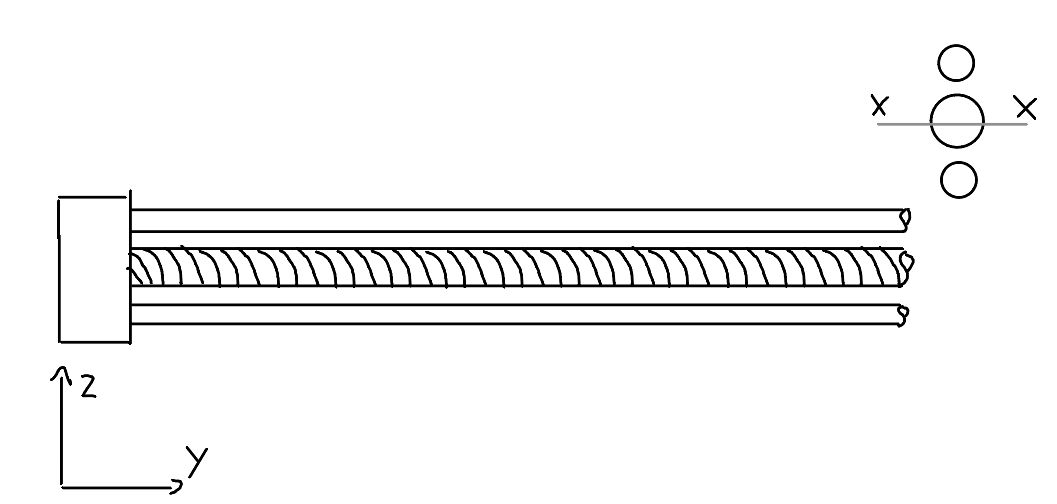
\includegraphics[width=\textwidth]{Sections/6 Detaljeløsning/Media/Tværsnit x-x.png}
        \caption{Tværsnit når følgestængerne er over hinanden} 
        \label{fig: Flytningsbidrag1}
    \end{subfigure}
    \hfil
    \begin{subfigure}[b]{0.5\textwidth}
    \centering
        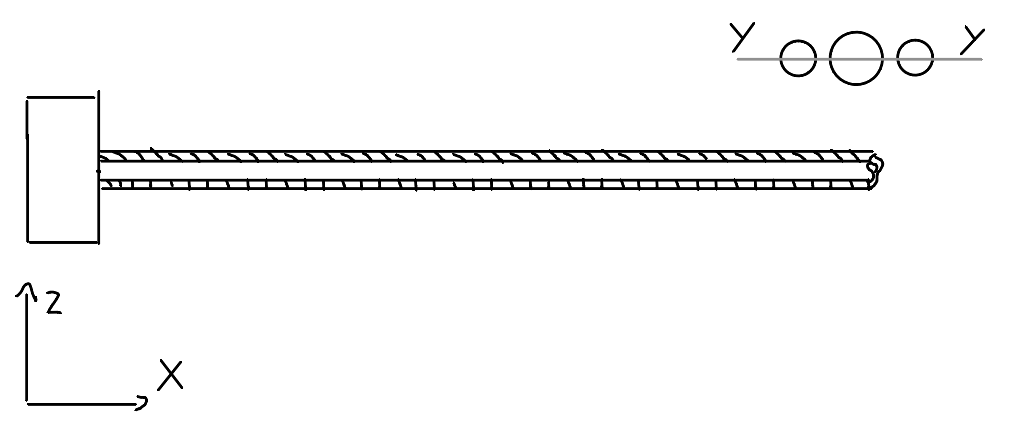
\includegraphics[width=0.9\textwidth]{Sections/6 Detaljeløsning/Media/Tværsnit y-y.png}
        \caption{Tværsnit når følgestængerne er ved siden af hinanden} 
        \label{fig: Flytningsbidrag2}
    \end{subfigure}
    \caption{Følgestængers placering i forhold til ledeskruen}
\end{figure}

Herfra ses der på hvilke kræfter som de lineære akser bliver udsat for. Aksernes egen masse samt punkmassen af PeJV'en vil vil have en lodret nedad rettet kraft. Derudover er der en kraft fra accelerationen og deaccelerationen af de lineære akser. Det vides at den nedadrettetede acceleration er tyngdeaccelerationen på $\SI{9,82}{m/s^2}$ og fra afsnit \ref{Kinematisk analyse} vides det at den lineære acceleration er på $\SI{70,8}{m/s^2}$. Dette betyder at det er denne laterale kraft som følgestængerne skal orienteres efter, da denne er størst. Derved skal følgestængerne være i den horisontale position for at modvirke bøjningen bedst og derved have den bedst mulige præcision. Flytningsbidraget afhænger af afstandsforskellen i bøjningsretningen i anden, i forhold til positionen af stængerne. Derfor afhænger flytningsbidraget af afstanden imellem stængerne i anden. 
\begin{figure} [H]
    \centering
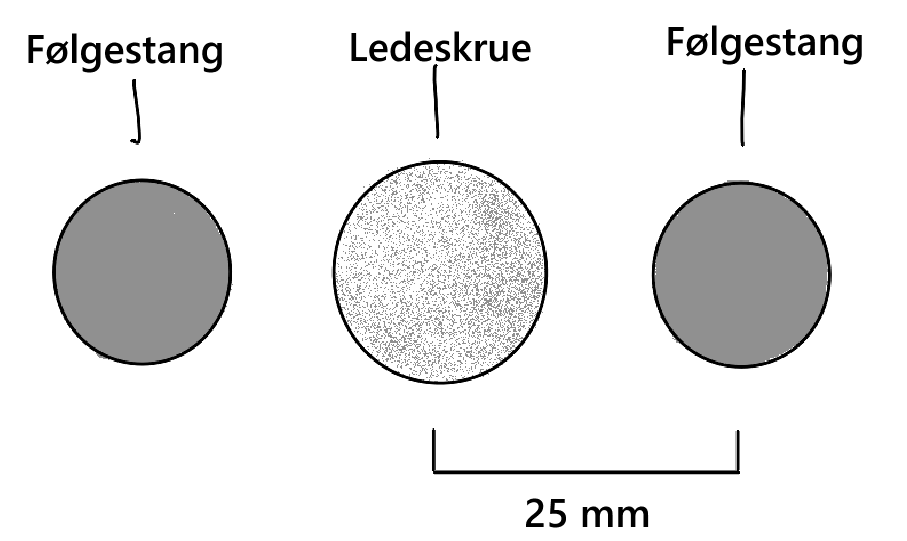
\includegraphics[width=0.5\linewidth]{Sections/6 Detaljeløsning/Media/Ledeskrue-afstand.png}
    \caption{Tværsnit af ledeskrue og følgestanger med indtegnet flytningsbidrag}
    \label{fig:flytningsbidrag}
\end{figure} \plainbreak{-.5}
For at give et betydeligt flytningsbidrag, er der valgt en afstand på $\SI{25}{mm}$ fra ledeskruens centrum, til følgestængernes centrum, se figur \ref{fig:flytningsbidrag}. Dette giver også plads til følgestængerne og ledeskruen, så de ikke rører hinanden.



\plainbreak{2}
\subsection{Vertikal udbøjning af ledeskrue} \label{Præcisions beregninger}
Designspecifikation 3 angiver at placeringen af en prik ikke må afvige mere end \(\SI{\pm0,1}{mm}\) fra punktet hvor prikken er angivet af softwaren. Denne præcision afhænger af motorens præcision, tolerancerne imellem ledeskruen og vognen, samt udbøjning af materialet ($W(y)$). Hvis stellet og bevægelsesdelene ikke har en tilstrækkelig stivhed vil der ske udbøjning, som resulterer i, en afvigelse af prikplaceringen. Det vælges at hovedet skal bevæges i alle 3 akser, fordi det vurderes at veje mindre end bundpladen og emnet. Dette giver mindre masse der skal flyttes, hvorved højere præcision kan opnås. Udbøjningen af den lineære y-akse i z-retningen kan bestemmes ved formel \ref{formel: udbøjning}.
\begin{equation} \label{formel: udbøjning}
    W(y)=\iint \frac{M(y)}{E \cdot I} dy^2
\end{equation}


\begin{figure}[H]
    \centering
    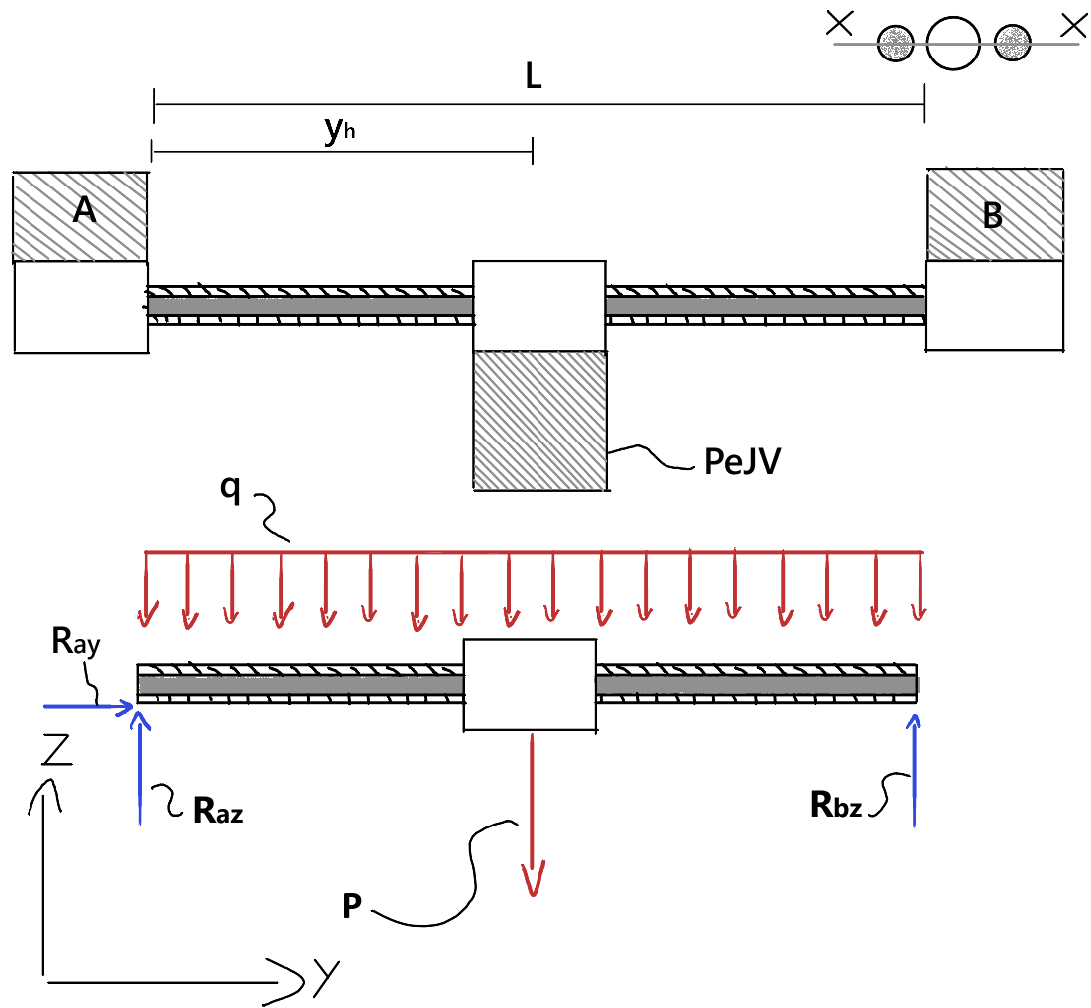
\includegraphics[width=0.6\linewidth]{Sections/6 Detaljeløsning/Media/FLD - y-akse.png}
    \caption{Fritlegeme diagram over y-aksen}
    \label{fig: FLD y-udbøj}
\end{figure}

Momentligningen ($M_{max}(y)$) er udledt fra bilag \ref{bilag- statik udledning} i formel \ref{formel: M_max(y)}. Denne formel er udledt af betingelserne fra figur \ref{fig: FLD y-udbøj}, hvor P's placering er uafhængig på stængerne. Ligningen for momentet indsættes i udbøjningsligningen \ref{formel: udbøjning}, hvilket giver \ref{formel: W(y)}
\begin{equation} \label{formel: W(y)}
    W(y)=\iint \frac{P\cdot \left(y-\frac{y^2}{L}\right)+\frac {q\cdot L}{2}\cdot\left( y-\frac{y^2}{L}\right)}{EI}dy^2
\end{equation}

Herefter dobbeltintegreres med hensyn til y:
\begin{equation} \label{formel: W_y med M og I}
   W(y)= \frac{P\cdot \left(\frac{y^3}{6}-\frac{y^4}{12\cdot L}\right)+\frac {q\cdot L}{2}\cdot\left(\frac{y^3}{6}-\frac{y^4}{12\cdot L}\right)}{EI} + C_1 y+C_2
\end{equation}

Da det er en simpel understøtning i begge ender af stængerne, indebærer det, at der ikke kan være en udbøjning i enderne. Dette giver randbetingelserne $W(0)=0$ og $W(L)=0$, der bruges til at finde konstanterne i \ref{formel: W_y med M og I}.
\begin{equation} \label{formel: W(0)}
        W(0)= \frac{P\cdot \left(\frac{0}{6}-\frac{0}{12\cdot L}\right)+\frac {q\cdot L}{2}\cdot\left(\frac{0}{6}-\frac{0}{12\cdot L}\right)}{EI} + C_1 0+C_2=0
\end{equation}

Når $y=0$ kræver det at $C_2=0$ for at opfylde kriteriet.
\begin{equation} \label{formel: W(L)}
       W(L)=\frac{P\cdot \left(\frac{L^3}{6}-\frac{L^4}{12\cdot L}\right)+\frac {q\cdot L}{2}\cdot\left(\frac{L^3}{6}-\frac{L^4}{12\cdot L}\right) }{EI} + C_1\cdot L=0
\end{equation} 

Ved $y=L$ fås $C_1=-\frac{P\cdot L^2}{12\cdot EI}-\frac{q\cdot L^3}{24\cdot EI}$. Disse konstanter indsættes i formel \ref{formel: W_y med M og I} for at få et endeligt udtryk for udbøjningen af stængerne.
\begin{equation} \label{formel: W(y) med C1 og C2}
   W(y)= \frac{P\cdot \left(\frac{y^3}{6}-\frac{y^4}{12\cdot L}-\frac{L^2\cdot y}{12}\right)+\frac {q\cdot L}{2}\cdot\left(\frac{y^3}{6}-\frac{y^4}{12\cdot L}-\frac{L^2\cdot y}{12}\right)}{E\cdot\frac{\pi}{2}\cdot r_f^4}
\end{equation}

For at holde præcisionen og farten i ledeskruen, er det nødvendigt at skruen ikke udbøjer mere end \(\SI{\pm0,1}{mm}\). Det er vurderet da en stor udbøjning resulterer i et spænd af skruen og følgestængerne. Det vælges at benytte følgestænger lavet i 1060 Carbon stål met et E-modul på omkring 200 GPa. For at undersøge sammenhængen imellem radius af følgestængerne og udbøjningen, plottes formel \ref{formel: W(y) med C1 og C2}. I denne formel og på dette plot, vil den maksimale udbøjning vurderes i forhold til radius af følgestængerne. Dette plot bruges til at finde, hvad radius skal være for at undgå \(\SI{\pm0,1}{mm}\) udbøjning.

\begin{figure}[H]
    \centering
    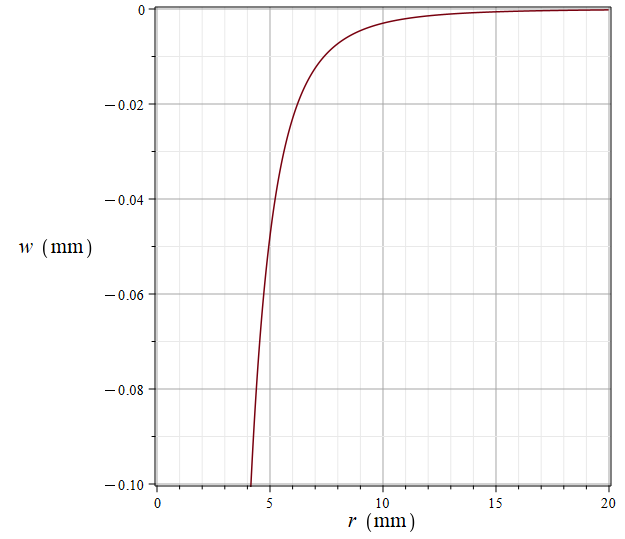
\includegraphics[width=0.7\linewidth]{Sections/6 Detaljeløsning/Media/Udbøjning ifht. r.png}
    \caption{Kurve for udbøjning på x-aksen, afhængigt af radius på følgestænger.}
    \label{fig: Udbøjninggraf}
\end{figure} \plainbreak{-0.5}

Af figur \ref{fig: Udbøjninggraf} fremgår det, at en radius på lidt over $\SI{4}{mm}$, vil opfylde kravet om mindre end $\SI{\pm 0,1}{mm}$ udbøjning. Under antagelserne, der er lavet omkring punktlastens placering, vurderes det at det værste tilfælde i forhold til udbøjning forekommer, når hovedet af prikværktøjet er så tæt på den ene af de lineære x-akser som muligt. Her vil kun ét af de to lineære x-akser bære hele hovedets vægt. Dette kan ikke lade sig gøre i virkeligheden, da hovedets dimensioner vil holde det fra, at være placeret lige under stængerne for den lineære x-akse. Dermed vil der i virkeligheden, altid være noget af vægten der holdes af stængerne på den anden side, hvilket betyder at det faktiske værste tilfælde er mindre udbøjet end der vises i formlen. Dette kan ses på figur \ref{fig: Udbøjningpraktik}.

\begin{figure}[H]
    \centering
    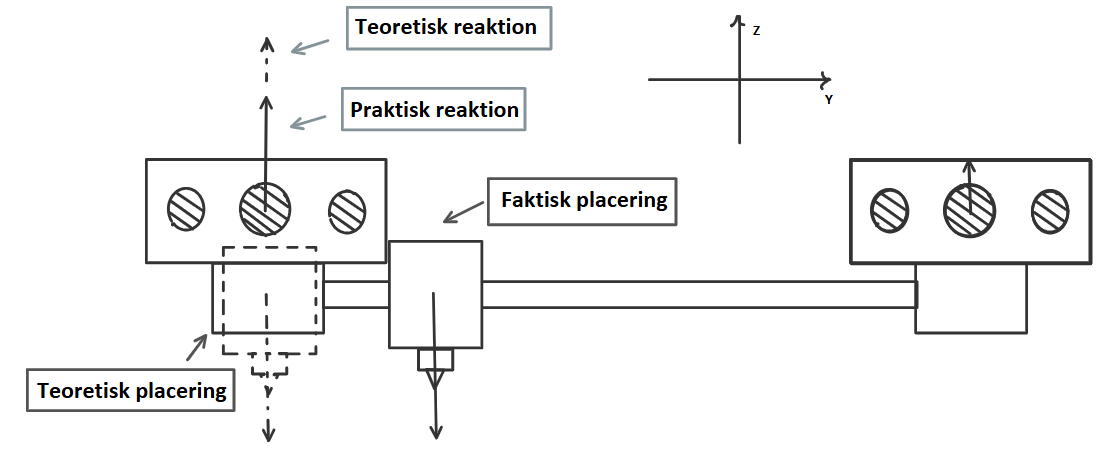
\includegraphics[width=0.9\linewidth]{Sections/6 Detaljeløsning/Media/Praktisk vs teoretisk udbøjning.png}
    \caption{Skitse af den teoretiske reaktion og den praktiske reaktion af de lineære x-akser.}
    \label{fig: Udbøjningpraktik}
\end{figure} \plainbreak{-0.5}

Dette betyder, at udregninger giver en sikkerhedsfaktor i forhold til virkelighedens udbøjning. Derudover er det også antaget, at ledeskruen ikke vil bære noget vægt, og i virkeligheden vil det ikke være muligt, og derfor vil den faktiske udbøjning også skulle bøje ledeskruen, som har en diameter på $\SI{10}{mm}$. Dette er også en sikkerhedsfaktor, og derfor vurderes kravet i forhold til maksimal udbøjning opfyldt.


\plainbreak{2}
\subsection{Udbøjning i xy-planet af ledeskrue}
I afsnit \ref{afs: Orientering af stænger} blev det klargjort at den største acceleration findes vinkelret på stængerne i xy-planet, når hovedet accelererer. Hovedets acceleration vil skabe en kraft grundet hovedets masse. Her vil flytningsbidraget være med til at modarbejde udbøjningen som nævnt i afsnit \ref{afs: Orientering af stænger}. Udbøjningen for stængerne i xy-planet, som resultat af disse kræfter udregnes. Dette gøres, for teoretisk at finde ud om løsningen lever op til præstationskrav 3. Formlen \ref{formel: I_xx med x^2 og A} angiver inertimomentet om z-aksen med flytningsbidraget. 
\begin{equation} \label{formel: I_xx med x^2 og A}
    I_{zz}=I_{zz1}+z^2\cdot A
\end{equation}

Her er $I_{zz}$ det samlede inertimoment, $I_{zz1}$ er inertimomentet uden flytningsbidrag, $z^2$ er højdeforskellen imellem arealmidtpunktet og hvert dels arealmidtpunkt og A er arealet af hver del. I dette tilfælde udbøjes om z-aksen i stedet for x- eller y-aksen, hvilket betyder flytningsbidraget afhænger af længde/bredde forskellen i anden fra arealmidtpunktet. Forskellen i bredde/længde af følgestængerne er \(\SI{50}{mm}\). Da de er lige store vil arealmidtpunktet være placeret med lige stor afstand i mellem dem og midten, altså \(\SI{25}{mm}\). Arealet er cirkulært og skrives derfor som $\pi \cdot r_f^2$.
\begin{equation}
    I_{zz}=I_{zz1}+y^2\cdot \pi\cdot r^2_f
\end{equation}

Kraften der påvirker udbøjningen vil være massen af hovedet ganget med dets acceleration. Denne kraft er fundet fra formel \ref{formel: Accelerationskraft}, og kan bruges igen i dette tilfælde. Udbøjningsligningen vil genbruges fra tidligere afsnit, da randbetingelserne og vilkårene er de samme i forhold til kraftens placering. I dette tilfælde skal inertimomentet og kraften opdateres til de nye værdier nævnt i dette afsnit.




\subsection{Opsummering på nøjagtgihed af prikplacering} \label{opsummering på nøjagtgihed af prikplacerin}


\renewcommand{\arraystretch}{1.1}
\begin{table}[H]
\setlength{\tabcolsep}{20pt}
 \centering
  \caption{Variabelliste}
 \begin{tabular}{|l c c|} \hline

  \multicolumn{3}{|c|}{\cellcolor{aaublue} \color{white} \textbf{NEMA 14 motor}}  \\\hline
 \rowcolor{gray!10}  \multicolumn{1}{|c}{\textbf{Beskrivelse}} & \multicolumn{1}{c}{\textbf{Symbol}}  & \multicolumn{1}{c|}{\textbf{Værdi}}  \\\hline
 Drejningsmoment af motor & \(\tau\) &\SI{0,12}{Nm}\\\hline
 Vinkelhastighed af motor & \(\omega\) & \SI{2000}{RPM}\\\hline
 Præcision af ledeskruen & \(\delta\) & \SI{0,01}{mm}\\\hline
 \specialrule{1pt}{0pt}{0pt}
 
  \multicolumn{3}{|c|}{\cellcolor{aaublue} \color{white} \textbf{Kinematik og statik}}  \\\hline
 \rowcolor{gray!10} \multicolumn{1}{|c}{\textbf{Beskrivelse}} & \multicolumn{1}{c}{\textbf{Symbol}} & \multicolumn{1}{c|}{\textbf{Værdi}}  \\\hline
  Tid pr. $\SI{}{cm^2}$ & \(t_{cm^2}\) & \SI{15,1}{s}\\\hline
  Acceleration & \(a\) & \SI{70,8}{m/s^2}\\\hline
  Radius af ledeskrue & \(r_l\) & \SI{5}{mm}\\\hline
  Gevindhældning af ledeskrue & \(O_l\) & \SI{2}{mm}\\\hline
  Radius af følgestænger & \(r_f\) & \SI{4}{mm}\\\hline
  Maksimal udbøjning & $W(y)_{max}$ & \SI{6,5d-3}{mm}\\\hline

 \end{tabular}
 \label{tab: variabelliste}
\end{table} \plainbreak{-.5}

Udbøjningen kommer til at være maksimalt $\SI{6,5d-3}{mm}$, og er dermed under kravet om $\SI{\pm0,1}{mm}$ afvigelse. Summen af tolerancerne fra udbøjningen og steppet i motoren må angive den samlede tolerance i forhold til præcision af prikplacering. Summen bliver $\SI{6,5d-3}{mm}+\SI{d-2}{mm}$ = $\SI{16,5d-3}{mm}$, hvilket er under afvigelsen på  $\SI{\pm0,1}{mm}$ med en faktor 6. Præstationskravet om prikpositionspræcision er derved opfyldt.